\documentclass[12pt]{article}
\usepackage[margin=1cm]{geometry}
\usepackage{polski}
\usepackage[utf8]{inputenc}
\usepackage{siunitx}
\usepackage{amsmath}
\usepackage{graphicx}
\usepackage{multicol}
\usepackage{nopageno}

\newenvironment{Figure}
  {\par\medskip\noindent\minipage{\linewidth}}
  {\endminipage\par\medskip}

\title{\textbf{Wahadło matematyczne - opracowanie danych}}
\author{Konrad Lewandowski}
\date{}

\begin{document}

\maketitle

\section{Metoda pierwsza}
\begin{multicols}{2}
Wyniki pomiarów długości:
\begin{align}
l &= 44.3 \si{\cm} \\
\Delta l &= 0.4 \si{\cm} \\
u(l) &= \frac{\Delta l}{\sqrt{3}} = 0.23 \si{\cm}
\end{align}
$l$ - zmierzona długość \\
$\Delta l$ - niedokładność pomiaru \\
$u(l)$ - niepewność pomiarowa długości
\\\\
Wyniki pomiarów czasu:
\\\\
\begin{center}
\begin{tabular}{|c|c|}
\hline
\textbf{Nr} & \textbf{10 $\cdot$ Czas [s]} \\
1 & 13.78  \\ \hline
2 & 13.28  \\ \hline
3 & 13.30  \\ \hline
4 & 13.38  \\ \hline
5 & 13.41 \\ \hline 
6 & 13.22 \\ \hline 
7 & 13.24 \\ \hline 
8 & 13.44 \\ \hline 
9 & 13.19 \\ \hline 
10 & 13.26 \\ \hline
\end{tabular}
\end{center}

\begin{align}
10\cdot\overline{T} & = 13.35 \si{\s} \\
\Delta T &= 268\si{\ms} \\
u(T) &= \sqrt{\frac{\sum\limits_{i=1}^{10}{(T_i - \overline{T})^2}}{90}} = 0.0055 \si{s}
\end{align}
$\overline{T}$ - średni czas \\
$\Delta T$ - niedokładność pomiaru (czas reakcji człowieka\footnote{http://www.humanbenchmark.com/tests/reactiontime/statistics}) \\
$u(T)$ - niepewność pomiarowa czasu

\columnbreak

\begin{Figure}
\centering
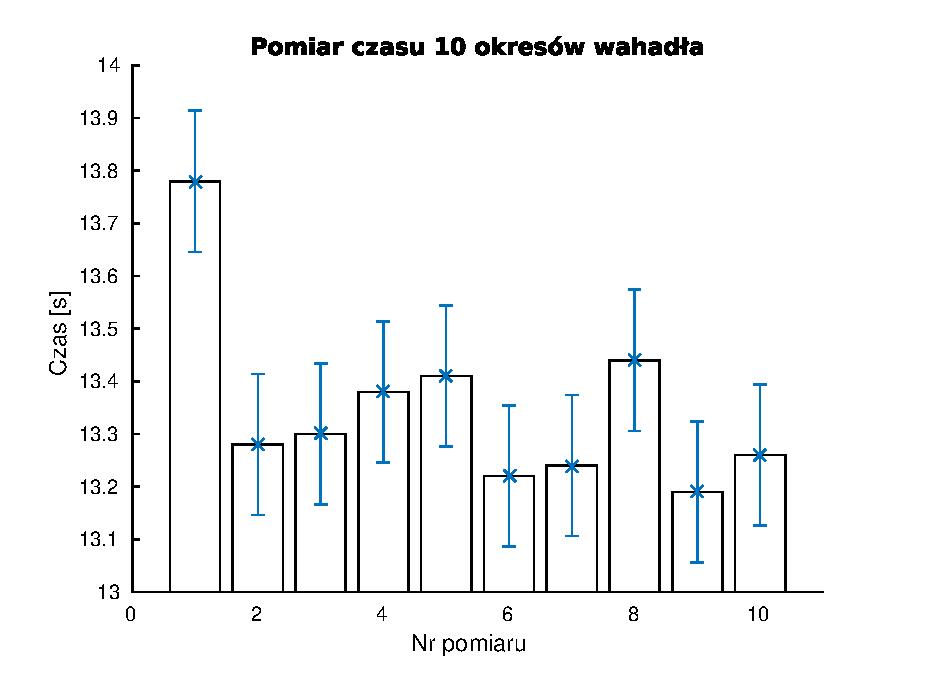
\includegraphics[width=\linewidth]{wykres.eps}
\end{Figure}

Obliczenie wartości g

\begin{align}
T &= 2 \cdot \pi \cdot \sqrt{\frac{l}{g}} \\
g &= 4 \cdot l \cdot \left( \frac{\pi}{T} \right)^2 \\
g &= 4 \cdot 0.443\si{\m} \cdot \left(\frac{3.1416}{1.335\si{\s}}\right)^2 = \textbf{9.813} \si{\frac{\m}{\s^2}} \\
u(g) &= \sqrt{\left(\frac{\partial g}{\partial l} \cdot u(l)\right)^2 + \left(\frac{\partial g}{\partial T} \cdot u(T)\right)^2} \\
&= \sqrt{\left(\frac{4\pi^2}{T^2}\cdot0.0023\right)^2+\left(-\frac{8 \pi ^2 l}{T^3}\cdot0.0055\right)} \\&= 0.096 \si{\frac{\m}{\s^2}}
\end{align}
$g$ - zmierzona wartość przyśpieszenia ziemskiego \\
$u(g)$ - niepewność pomiarowa przyśp. ziemskiego
\begin{equation}
B(g) = g - g_0 = 9.813 - 9.80665 = \textbf{0.00635}\si{\frac{\m}{\s^2}}
\end{equation}
$B(g)$ - błąd pomiaru \\
$g_0$ - standardowa wartość przyśpieszenia ziemskiego
\end{multicols}
\newpage

\section{Metoda druga}
\begin{multicols}{2}
\begin{Figure}
\centering
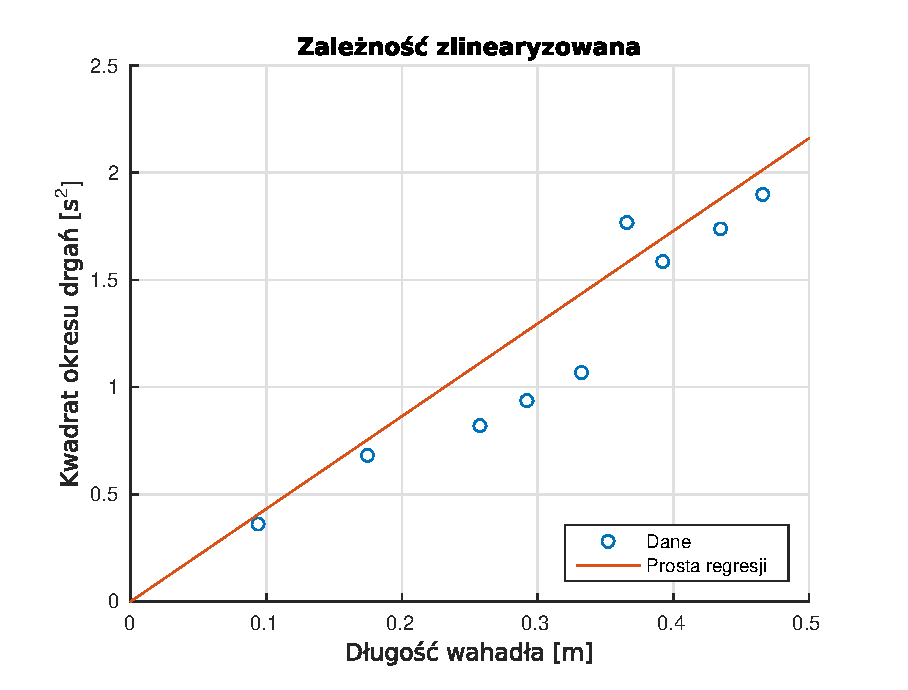
\includegraphics[width=\linewidth]{wykres2.eps}
\end{Figure}

\begin{align}
a&= 4.32\si{\frac{\s^2}{\m}} \\
u(a)&= 0.53\si{\frac{\s^2}{\m}}  \\
g&=\frac{4 \cdot \pi^2}{a} = \textbf{9.14}\si{\frac{\m}{\s^2}} \\
u(g) &= \sqrt{ \left(\frac{\partial g}{\partial a} \cdot u(a)\right)^2}
= 1.11\si{\frac{\m}{\s^2}}
\end{align}
$a$ - współczynnik regresji\footnote{Parametry regresji obliczyłem korzystając z pakietu R}\\
$u(a)$ - niepewność pomiarowa regresji\\
$g$ - obliczona wartość przyśpieszenia ziemskiego \\
$u(g)$ - niepewność pomiarowa przyśp. ziemskiego
\columnbreak
\\
Wyniki pomiarów: \\
\\
\begin{tabular}{|c|c|c|}
\hline
Nr & Długość [cm] & 10 $\cdot$ Czas [s] \\ \hline
1  & 36.6         & 12.29    \\ \hline
2  & 29.2         & 9.68     \\ \hline
3  & 33.2         & 10.35    \\ \hline
4  & 25.7         & 9.04     \\ \hline
5  & 17.4         & 8.25     \\ \hline
6  & 9.4          & 6.03     \\ \hline
7  & 4.66         & 13.77    \\ \hline
8  & 43.5         & 13.18    \\ \hline
9  & 39.2         & 13.60    \\ \hline
\end{tabular}
\end{multicols}

\end{document}